{
\subsection{Pełna treść pytania}
Dla porządku -- podajmy pełną treść pytania, bo była zbyt długa by ją dać do nazwy sekcji.

\begin{question}[Proces Poissona]
 Definicja i potrzebne własności aby wykazać co następuje. Niech \((N(t),t_0)\) będzie procesem Poissona o parametrze \(\lambda\). Wykazać, że jeśli w przedziale czasowym \((0,t]\) zaszło dokładnie jedno zdarzenie, czyli \(N(t) = 1\) to czas zajścia tego zdarzenia \(X_1\) ma rozkład jednostajny na przedziale \((0,t]\) (w szczególności nie zależy od \(\lambda\)).
\end{question}

\makeatletter
\def\input@path{{../probabil}}
\makeatother
\graphicspath{{../probabil}}

% This has to be done, because we input another suffering with different sectioning scheme.
\let\realsection\section
\let\realsubsection\subsection
\let\section\subsection
\let\subsection\subsubsection
\let\subsubsection\paragraph

\realsubsection{Podstawowe własności procesu Poissona}
\begin{definition}
    Definiujemy rozkład normalny (uogólniony) jako rozkład o następującej funkcji gęstości prawdopodobieństwa: 

    \[ f_Z(z) =  \frac{1}{\sigma\sqrt{2\pi}}e^{-((z - \mu)/\sigma)^2/2} \]
\end{definition}

\begin{definition}
    Rozkład normalny o parametrach \(\mu\) i \(\sigma^2\) oznaczamy jako \(N(\mu , \sigma^2 )\).
\end{definition}

\begin{definition}
    Standardowy rozkład Normalny to rozkład normalny o parametrach \( \mu = 0\) i \( \sigma^2 = 1\); oznaczamy go (bez większego szoku) jako \(N(0, 1)\).
\end{definition}

\begin{definition}
    Dystrybuantę standardowego rozkładu normalnego oznaczamy jako \( \Phi \).
\end{definition}

Funkcja gęstości prawdopodobieństwa standardowego rozkładu normalnego wygląda jak \sout{dzban} dzwon.

\begin{center}
    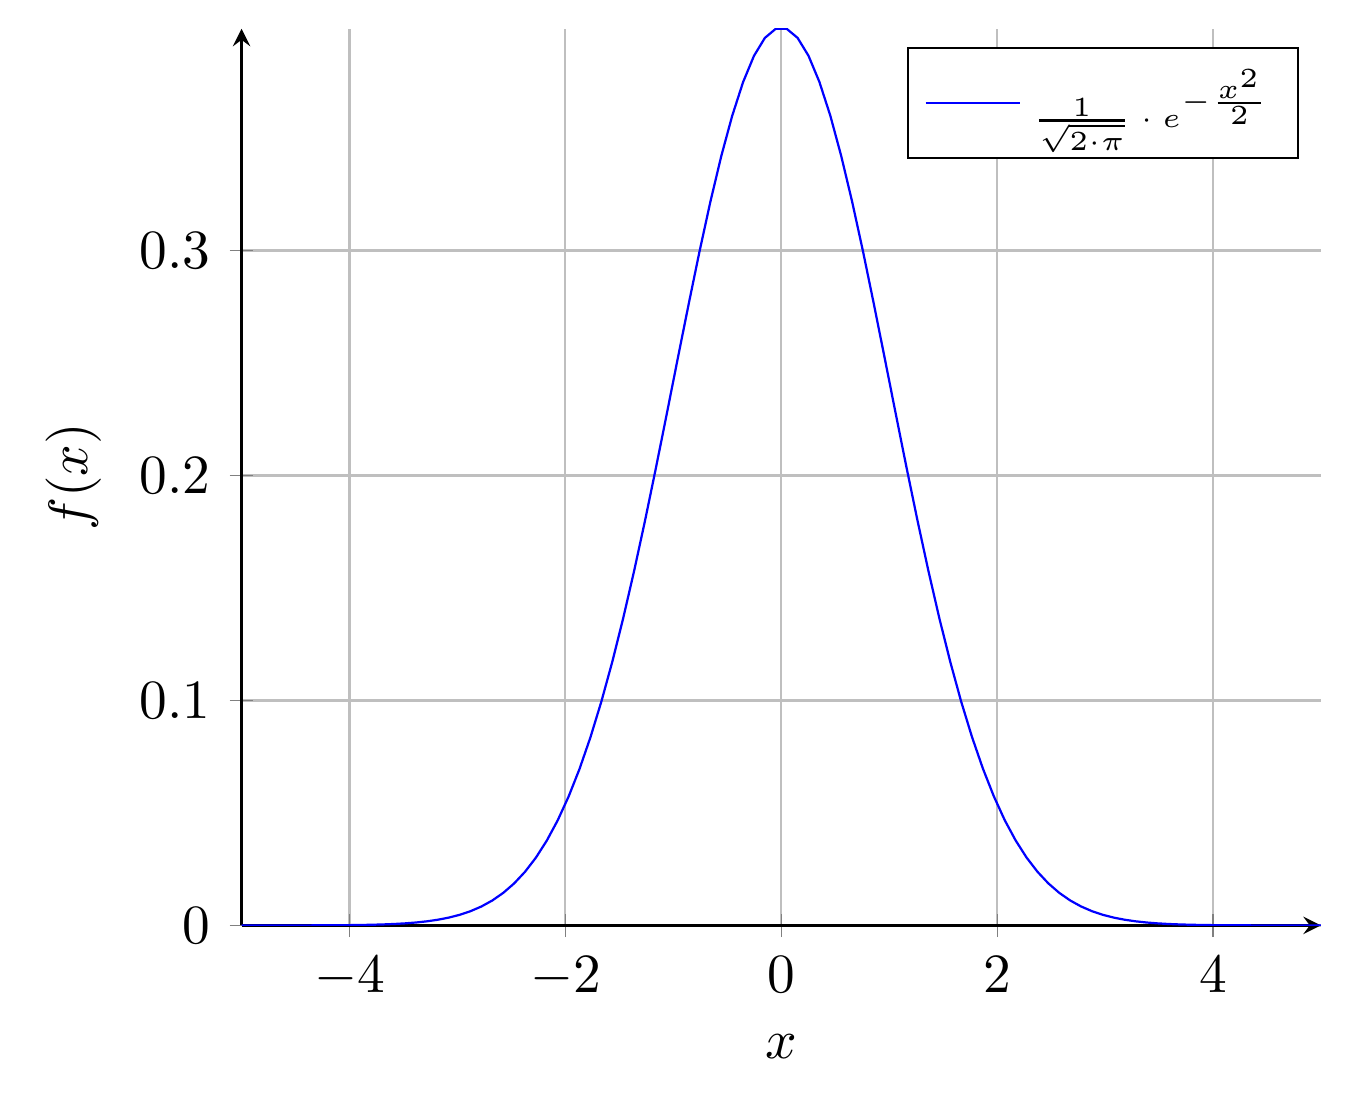
\begin{tikzpicture}[scale=2]
    \begin{axis}[
        axis lines = left,
        xlabel = \(x\),
        ylabel = {\(f(x)\)},
        ymajorgrids = true, 
        xmajorgrids = true,
    ]
    \addplot [
        domain=-5:5, 
        samples=100, 
        color=blue,
    ]
    {(1/sqrt(2*pi)) * e^(-x^2/2)};
    \addlegendentry{\tiny \(\frac{1}{\sqrt{2 \cdot \pi}} \cdot e^{-\frac{x^2}{2}}\)}
 
    \end{axis}
    \end{tikzpicture}    
\end{center}


\realsubsection{Warunkowe czasy zdarzeń}
Możemy teraz przejść do udowadniania tego, co zostało nam nakazane w pytaniu (ale super)! 

Wyobraźmy sobie zatem sytuację, gdzie w przedziale czasowym \((0, t]\) doszło do jakiegoś zdarzenia. Policzmy sobie prawdopodobieństwo, że w przedziale \((0, s]\) (dla jakiegoś \(s \leq t\)) \textit{nie} doszło do tego zdarzenia. 

Uwaga techniczna: jak będziemy teraz notować rzeczy typu \(N(s)\) lub \(N(t)\) będziemy mieli na myśli \textit{ten sam proces}, a jako że przedziały których ,,dotyczą'' te zmienne losowe się pokrywają to będą one od siebie zależne. 

No to jedziemy z tematem. 

\begin{align*}
    \p(N(s)=0 | N(t)=1) &= \frac{\p(N(s)=0 \land N(t)=1)}{\p(N(t)=1)}  \\
    &= \frac{\p(N(s)=0 \land N(t-s)=1)}{\p(N(t)=1)}
\end{align*}

Tutaj uwaga: \(N(s)\) i \(N(t-s)\) będą już od siebie niezależne, bo te zmienne mają na celu opisywać niezależne od siebie przedziały. Tym samym możemy kontynuować nasze obliczenia:

\begin{align*}
    \frac{\p(N(s)=0 \land N(t-s)=1)}{\p(N(t)=1)} &= \frac{\p(N(s)=0) \cdot \p(N(t-s)=1)}{\p(N(t)=1)}  \\
    &= \frac{e^{-\lambda s} \cdot \lambda (t-s) e^{-\lambda (t-s)}}{\p(N(t)=1)} \\ 
    &= \frac{e^{-\lambda s} \lambda (t-s) e^{-\lambda t + \lambda s}}{\p(N(t)=1)} \\ 
    &= \frac{\lambda (t-s) e^{-\lambda t}}{\p(N(t)=1)} \\
    &= \frac{\lambda t e^{-\lambda t} - \lambda s e^{-\lambda t}}{\p(N(t)=1)} \\ 
    &= \frac{\lambda t e^{-\lambda t} - \lambda s e^{-\lambda t}}{\lambda t e^{-\lambda t}} \\
    &= 1 - \frac{\lambda s e^{-\lambda t} }{\lambda t e^{-\lambda t}} \\ 
    &= 1 - \frac{s}{t}
\end{align*}

Czyli całkiem ewidentnie mamy tutaj do czynienia z rozkładem jednostajnym; w szczególności całkowicie obojętny jest mu parametr \(\lambda\) (co było do przewidzenia bo to rozkład jednostajny, ya know). 

Żeby być całkowicie formalnymi w wykazaniu że to jest rozkład jednostajny to zdefiniujmy sobie zmienną losową \(X\) która jako wartość przyjmuje dokładny czas zdarzenia. 

Widzimy, że dla \( a \in (0, t]\):

\[ 
    \p(X < a) = \p(N(a)=0 | N(t)=1) = 1 - \frac{s}{t}
\]

Zatem dystrybuanta jest taka:

\[
    F_X(a) = \p(X \geq a) = 1 - \p(X < a) = 1 - 1 + \frac{s}{t} = \frac{s}{t}
\]

Czyli dystrybuanta zmiennej \(X\) jest taka sama jak dystrybuanta zmiennej losowej rozkładu jednostajnego, a to kończy dowód. 

}